\clearpage
\section{Conceitos Gerais}
\label{ch:background}

Esta seção descreve brevemente conceitos e background tais como o paradigma Névoa/Nuvem multinível e Serviço de Video Streaming.
%This section briefly introduces background and concepts such as the \acl{SDN} paradigm and the 4G \acl{LTE} networks.

%=============================================================================%
\subsection{Computação em Névoa}

A computação em névoa tem como principal objetivo preencher uma lacuna entre a nuvem e os dispositivos finais. Existem várias definições e terminologias na literatura que abordam este paradigma na literatura. Nesta proposta, vamos adotar a definição, o qual é adotado pelo OpenFogConsortium~(OpenFog), publicada pelo Instituto Nacional da Padrões e Tecnologia%\textit{National Institute of Standards and Technology}
~(NIST)~\cite{NIST2018-FogComputingConceptualModel}: 

\begin{displayquote}

"\textit{A computação em névoa é um modelo em camadas para permitir o acesso onipresente a um contínuo compartilhado de recursos de computação escalonáveis. O modelo facilita a implantação de aplicativos e serviços distribuídos com reconhecimento de latência e consiste em nós de névoa (físicos ou virtuais), que residem entre dispositivos finais inteligentes e serviços centralizados (na nuvem)}."

\end{displayquote}
% https://nvlpubs.nist.gov/nistpubs/SpecialPublications/NIST.SP.500-325.pdf. March 2018
% https://www.openfogconsortium.org

Os nós podem ser organizados em arquiteturas multiníveis - na vertical (para dar suporte ao isolamento), na horizontal (para suportar a federação) ou pela latência entre os nós da névoa e os usuários finais. A computação em Névoa minimiza o tempo de resposta das aplicações suportadas e fornece, para os dispositivos finais, recursos de computação local e, quando necessário, conectividade de rede para serviços centralizados. %Os nós da \textit{fog} são recursos locais que podem ser organizados em arquiteturas multi-níveis e podem ser quaisquer dispositivos que oferece conexão de rede com fio/sem fio com computação, armazenamento e conectividade de rede, como switches, roteadores, smart phones, tablets, laptops, etc. 

%---------------------------------------------------------------------
\subsection{Arquitetura Multinível em Névoa/Nuvem}


Uma arquitetura em névoa verticalmente com N níveis tem como proposito: 
\textit{i)} Aprimorar o QoE dos usuários, servindo o conteúdo solicitado de borda o mais próximo possível do usuário;
\textit{ii)} Reduzir o congestionamente no core da rede, pois representa uma sobrecarga operacional para o adiministrador da rede;
\textit{iii)} lidar eficientemente com a quantidade de dados que precisa ser processada e extrair dados significativos para criar mais inteligência em cada nível. 
%  (iii) O tráfego enviado entre a origem e a hierarquia de servidores deve ser reduzido, pois incorre em custos para os provedores de conteúdo. 
%
%Além disso, o número de camadas afeta diretamente o suporte de QoE.
%to deal efficiently with the amount of data that needs to be processed and to extract meaningful data to create more intelligence at each level. Moreover, the number of tiers impacts direclty in the QoE support.
%O OpenFog está assumindo a liderança na padronização de névoa e definiu uma arquitetura de referência que consiste em N camadas de nós, como mostra a Figura~\ref{fig:arch-multi-lvl}

Primeiramente, vamos apresentar uma arquitetura de rede com multiníveis, detalhada na Figura~\ref{fig:arch-multi-lvl}. O nível superior é composto por servidores em nuvem que podem ser localizados em um setor público ou privado. As nuvens podem ser qualquer provedor do streaming de video, por exemplo, Netflix, Amazon ou Youtube, bem como, um usuário local. % Estas nuvem operam o conteudo multimidia original sobre redes WANs.
Os 3 níveis seguintes representam a rede névoa/nuvem organizada hierarquicamente. Este  trabalho leva em consideração os nós da borda com serviços de armazenamento e computação, bem como, é ranqueado de acordo com a área de cobertura de comunicação. Nesse ecossistema multinível, o \textit{Core Network Regional Edge} pode gerenciar a coordenação em toda a cidade, por exemplo, unidade de banda de base~(BBU) ou provedor de serviços de Internet~(ISP). Seguido pela \textit{Access Network Edge}, que suporta algumas dezenas a talvez algumas centenas de nós locais no meio da nevoa, por exemplo, estação base ou ponto de acesso. Os \textit{Gateways} de borda podem ser distribuídos em nós de névoa locais, por exemplo, computadores pessoais, laptops e smartphones, onde o nó retransmite o conteúdo do vídeo por meio de comunicação com ou sem fio. Esses dispositivos têm demandas de tráfego altas e similares, podendo cooperar entre si.% Essa conexão é feita através de algum tipo de rede local~(LAN). 
%É importante notar que em um ambiente multinível os servidores são organizados em uma topologia mesh em arvore.
\vspace{0.8cm}
\begin{figure}[htb]
  \centering
  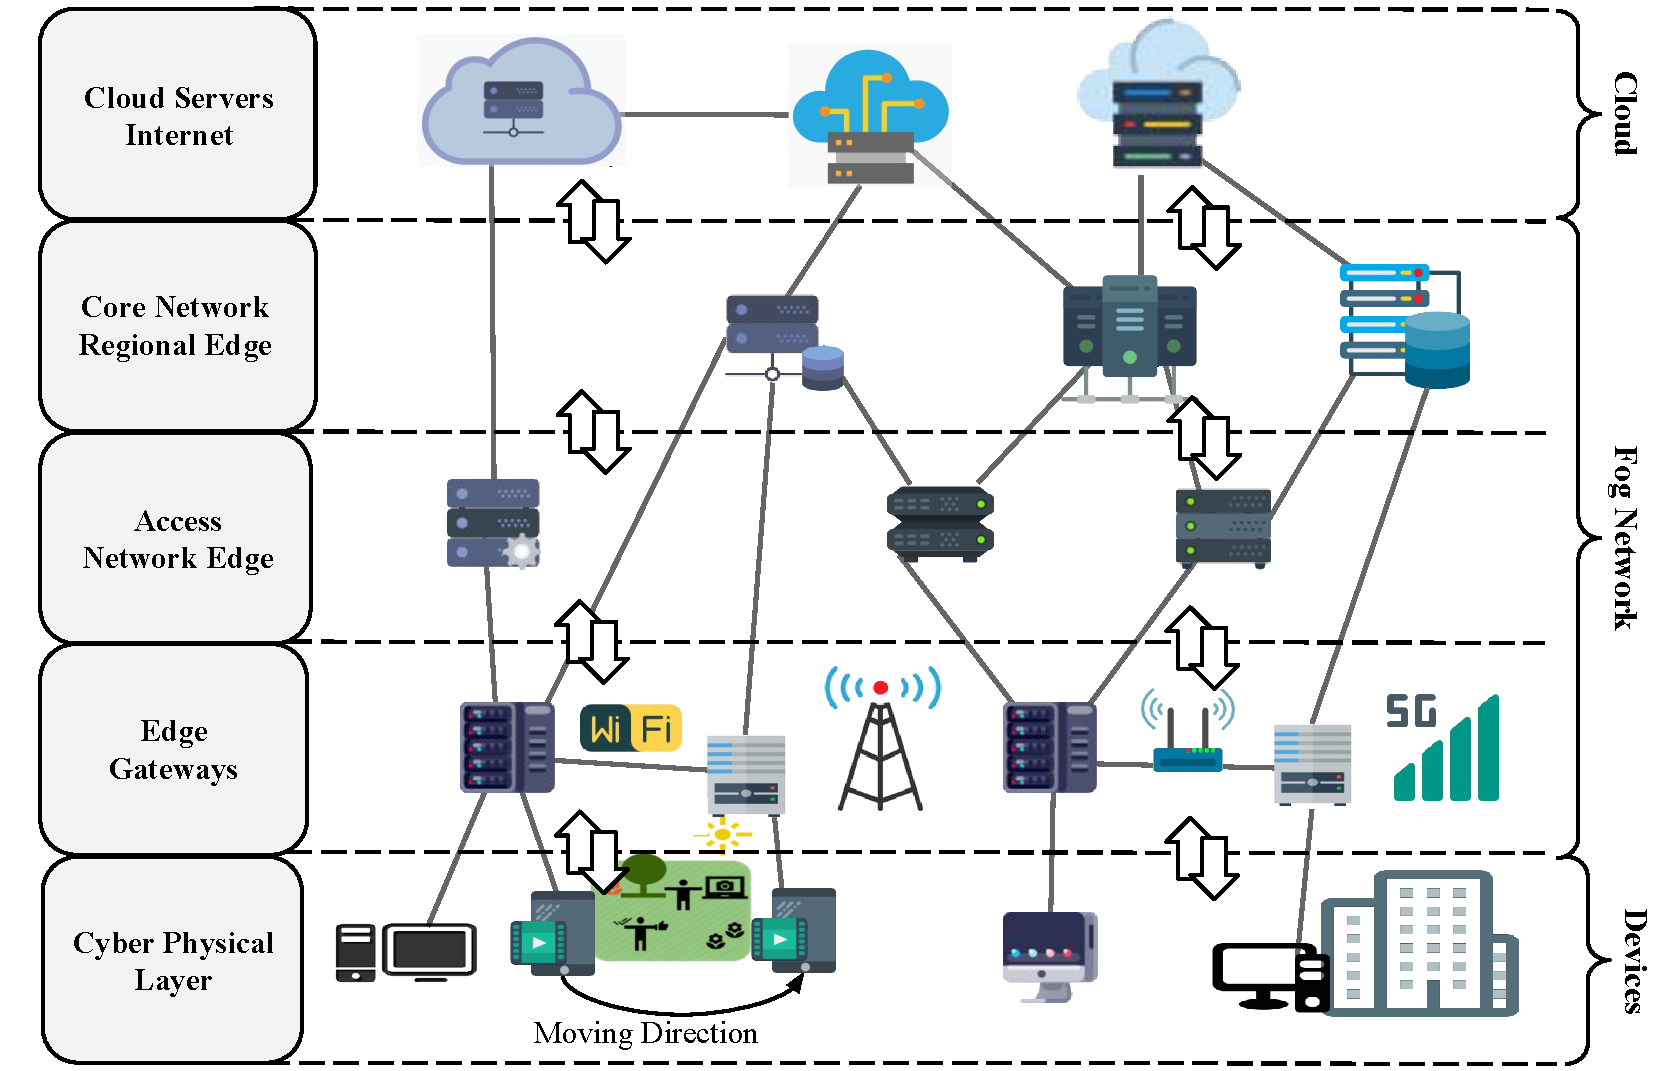
\includegraphics[scale=.45]{arch-multi-lvl}
  \caption{Visão geral do ambiente multinível Névoa/Nuvem.}
  \label{fig:arch-multi-lvl}
\end{figure}

%Um cenário simples é que um shopping center pode implantar muitos nós de névoa em diferentes andares para fornecer Acesso Wi-Fi e entregar alguns serviços envolvidos (ou seja, navegação interior, distribuição de anúncios, coleções de feedback) para seus clientes. No entanto, no tempo de pico, as capacidades desses nós de nevoeiro não podem servir eficientemente os clientes. Enquanto isso, o provedor de névoa, aqui é o centro comercial, pode estender sua infraestrutura, pagando os recursos de computação e armazenamento terceirizados dos nós de nuvem, que pode ser máquina virtual (VM) alugada de provedores de nuvem em uma base de pay-per-use. Todos os nós de processamento distribuídos (nuvem ou névoa) são gerenciados por um corretor de recursos, que é um componente de gerenciamento de recursos e um planejador para os fluxos de trabalho enviados pelos usuários no lado do nevoa. 
%Neste caso, uma agenda de tarefas, que pode minimizar o tempo de conclusão do fluxo de trabalho, mas corresponde a uma grande quantidade de custo monetário, não é uma solução ideal para fornecedores da fog. 
%Assim, neste artigo, propomos um algoritmo de escalonamento de tarefas que pode conseguir uma boa compensação entre o tempo de execução do fluxo de trabalho e o custo pelo uso dos recursos da nuvem. Os resultados experimentais mostram o excelente desempenho do nosso método comparado com alguns outros trabalhos.	

%Com novas possibilidades sendo criadas para oferecer melhores serviços e o funcionamento da internet. Enquanto a rede se torna mais robusta, o problema se torna mais complexo e surgem novos desafios. Para adaptar um sistema CDN com ambiente de várias camadas ao nevoeiro, diferentes características devem ser estudadas, como alocação de cache, posicionamento, substituição e seleção, geralmente, tomada de decisões em tempo real. Como diferentes tamanhos de cache, sendo alocados nas camadas para armazenar um intervalo de conteúdo para provisionar uma região. Além disso, um tamanho de cache em um dispositivo AP deve ser capaz de lidar com um conjunto de diferentes partes de conteúdo, para que os usuários finais possam ter garanias de QoE. Assim, surge um nível diferente de granularidade nos dispositivos de ponto de acesso. Se a granularidade de certas áreas se tornar muito granularidade, problemas de escalabilidade começam a aparecer. Dividir o conteúdo do nevoeiro na rede pelos APs no nível certo de granularidade é um problema complexo por si só.

%-----------------------------------------------------------------------------%
%\subsection{HTTP Adaptative Streaming and MPEG-DASG standard}
\subsection{Transmissão Adaptativa de vídeo pela Internet}
\label{sec:has-dash}

A padronização de uma arquitetura HAS prove importantes benefícios sobre sistemas de streaming tradicionais. Devido ao fato de várias empresas importantes de mídia participarem de seu desenvolvimento, este novo protocolo elimina problemas técnicos na entrega e compactação do video. Em essência, o objetivo é combinar todas as tecnologias e padrões em um, tornando o suporte a streaming contínuo em todos os dispositivos. 
%Por sua vez, visa reduzir dores de cabeça técnicas e custos de transcodificação. 
Os editores de conteúdo podem gerar um único conjunto de arquivos para codificação e streaming que deve ser compatível com o maior número possível de dispositivos, do smartphone a nuvem, além de plug-ins ou HTML5. Os consumidores não precisam se preocupar se seus dispositivos conseguem reproduzir o conteúdo que desejam assistir.

O objetivo desses esquemas é garantir um alto QoE para os usuários na presença de flutuações na largura de banda devido a alguns fatores, por exemplo, controle de congestionamento da rede, intensidade do sinal, perda de pacotes e assim por diante. Embora essas flutuações sejam bastante comuns na Internet pública, elas também podem ocorrer em redes mais privadas, como redes domésticas ou mesmo redes gerenciadas, onde geralmente há controle de admissão e diferentes ferramentas de QoS são usadas. 

% Quality Improvement for HTTP Adaptive Streaming over Mobile Networks Hung Thai Le
%To deliver videos over the Internet, the MPEG-2 transport stream (M2TS) [74] and ISO Base Media File Format (MP4) [75] are popularly used [22]. In HAS, we only consider transmissions of video segments at the application layer. After obtaining the metadata file, the client issues a series of HTTP requests to download video segments, typically in chronological order, selecting a representation for each ofthem from the set ofavailable representations.
%Para entregar vídeos pela Internet, o fluxo de transporte MPEG-2 (M2TS) [74] e o formato ISO de arquivo de mídia básico (MP4) [75] são usados popularmente [22]. No HAS, consideramos apenas transmissões de segmentos de vídeo na camada de aplicação. Após obter o arquivo de metadados, o cliente emite uma série de solicitações HTTP para baixar segmentos de vídeo, geralmente em ordem cronológica, selecionando uma representação para cada um deles no conjunto de representações disponíveis.
%
%As aplicações de video streaming baseadas em MPEG-DASH, uma tecnologia que se adapta dinamicamente às mudanças nas condições da rede, solicitando conteúdo em segmentos codificados com taxas de bits diferentes e que é usada pelos principais serviços de streaming como Netflix e YouTube.
%a technology that dynamically adapts to changing network conditions by requesting content in chunks encoded at different bitrates, and which is used by major streaming services like Netflix and YouTube.
%In this proposal, we focus on video streaming applications based on MPEG-DASH (Dynamic Adaptive Streaming over HTTP), a technology that dynamically adapts to changing network conditions by requesting content in chunks encoded at different bitrates, and which is used by major streaming services like Netflix and YouTube.
%There are several key benefits in the adaption of this new standard. Due to the fact that several major media companies took part in its development, the new protocol will eliminate technical issues in delivery and compression. In essence, it aims to combine all of the technologies and standards into one, making streaming support seamless on all devices. In turn, it aims to reduce technical headaches and transcoding costs. Content publishers can generate a single set of files for encoding and streaming that should be compatible with as many devices as possible, from mobile to OTT, as well as to the desktop via plug-ins or HTML5. Consumers will not have to worry about whether their devices will be able to play the content they want to watch.

\vspace{0.5cm}
\begin{figure}[htb]
  \centering
  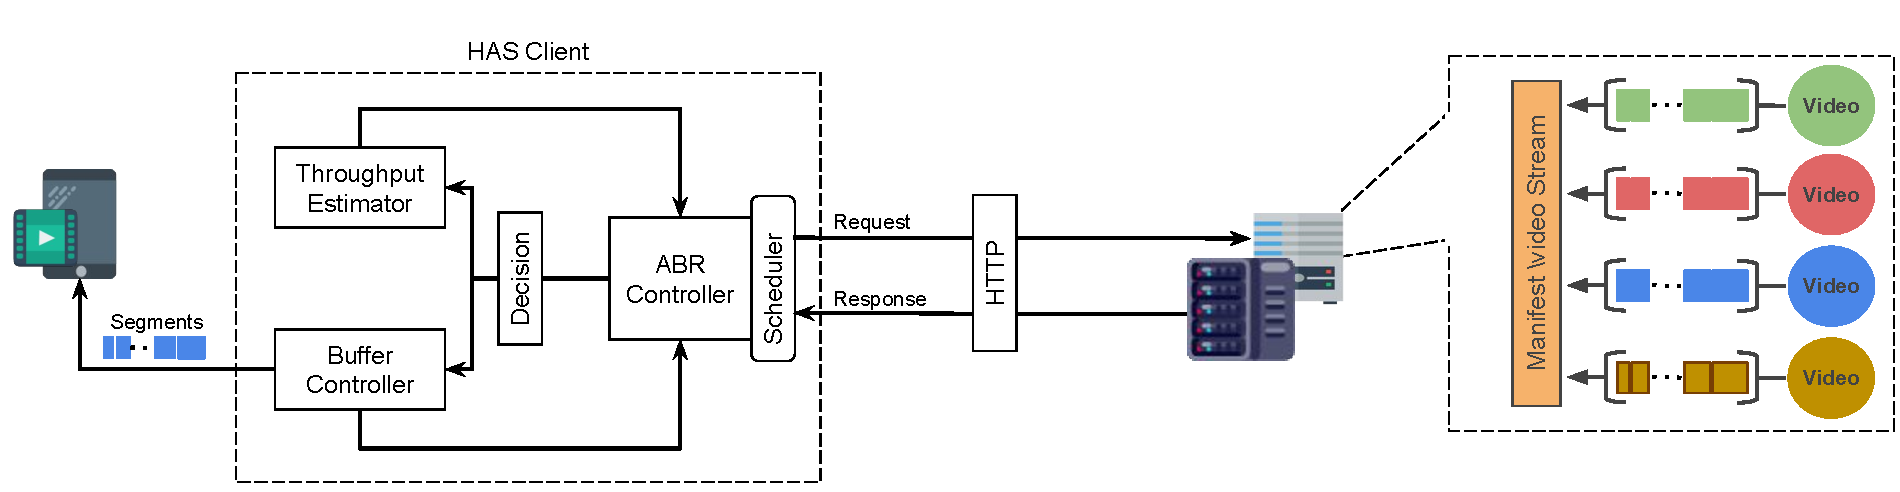
\includegraphics[scale=.5]{has-arch}
  \caption{Arquitetura de distribuição HAS.}
  \label{fig:has-arch}
\end{figure}

%By parsing the MPD, the DASH client learns about the program timing, media-content availability, media types, resolutions, minimum and maximum bandwidths, and the existence of various encoded alternatives of multimedia components, accessibility features and required digital rights management (DRM), media-component locations on the network, and other content characteristics. 
%Ao analisar o arquivo MPD, o cliente DASH aprende sobre o tempo do programa, disponibilidade de conteúdo de mídia, tipos de mídia, resoluções, larguras de banda mínima e máxima e a existência de várias alternativas codificadas de componentes de multimídia, localizações dos componentes de mídia na rede e outras características do conteúdo
%
%Out of Scope
%The MPEG-DASH specification only defines the MPD and the segment formats. The delivery of the MPD and the media encoding formats containing the segments, as well as the client behavior for fetching, adaptation heuristics, and playing content, are outside of MPEG-DASH’s scope.

Na Figura~\ref{fig:has-arch}, conforme ilustrado, o cliente e servidor HAS usam o protocolo HTTP na camada da aplicação para realizar todas as requisições/respostas necessárias. 

No lado do servidor, assim que um arquivo de mídia~(ou fluxo) estiver pronto, ele será preparado para transmissão antes de ser publicado em um servidor HTTP padrão. O arquivo/fluxo original é particionado em segmentos~(também chamados de \textit{chunks}) de tempo de reprodução equivalente, e são geradas várias versões (também chamadas de representações) de cada segmento que variam em taxa de bits/resolução/qualidade usando um codificador ou um transcodificador. 
Além disso, o servidor gera um arquivo manifesto chamado de descritor da apresentação na mídia~(MPD), que lista as representações disponíveis, incluindo informações como o tempo do video, disponibilidade de conteúdo, tipos de mídia~(ou seja, H.264, H.265, etc.), resoluções, larguras de banda mínima e máxima e a existência de várias alternativas codificadas de componentes de multimídia, localizações dos segmentos de mídia na rede e outras características do conteúdo.
%URLs para identificar os segmentos e seus tempos de disponibilidade. 

No lado do cliente HAS, primeiramente, o reprodutor de video solicita o manifesto ao servidor HTTP e analisa as informações citadas acima. Desta forma, ele pode começar a solicitar segmentos sequencialmente e adaptar-se às condições da rede dinamicamente usando sua lógica adaptativa de taxa de bits~(ABR). Os esquemas ABR também levam em consideração o buffer de reprodução, recursos do dispositivo, preferências do visualizador, além de recursos de conteúdo, com pesos diferentes. 
Como a QoE do espectador precisa ser determinado em tempo real durante a reprodução, geralmente, são usadas métricas objetivas, incluindo o número de interrupções, duração do atraso na inicialização, frequência e quantidade de oscilações de qualidade do vídeo. Por padrão, o HAS não exige nenhum esquema de adaptação específico, deixando aos desenvolvedores de sistemas inovar e implementar seu próprio método.


%O analisa o MPD arquivo MPD , o player do cliente extrai 
%Em seguida, as soluções HAS realizam a adaptação dinâmica em relação às estas variaveis para fornecer uma experiência de streaming contínua~(ou pelo menos mais suave). 

%Durante uma sessão HAS atípica, o cliente recebe primeiro o manifesto que contém os metadados para vídeo, áudio, legendas etc. e depois mede constantemente certos parâmetros, como largura de banda de rede disponível, status do buffer e níveis de bateria e CPU. De acordo com esses parâmetros, o cliente HAS busca repetidamente o próximo segmento mais adequado entre as representações disponíveis do servidor.
%A Tabela 1.1 compara as principais características dos sistemas tradicionais de streaming e HAS.

%-----------------------------------------------------------------------------%
%\subsubsection{Arquitetura Hierarquica para Bitrate Schemes}
%\label{subsec:bitrate-schemes}
%
%%Implementing a multi-tier architecture has a dual purpose: to deal efficiently with the amount
%%of data that needs to be processed and to extract meaningful data to create more intelligence at
%%each level. Moreover, the number of tiers impacts direclty in the QoE support.
%
%Each ABR scheme proposes many criteria for bitrate decisions, where they work only under
%indirect or implicit assumptions and specific scenarios, and focuses on a specific deployment or
%different network characteristics. Currently, there is a lack of a general consistent framework
%that can formally evaluate and compare different bitrate adaptation schemes, and test and
%verify the efficiency of their components. To the best of our knowledge, only a few algorithms
%formally describe what objective they want to optimize, and thus, it is challenging to make
%an effective comparison.
%
%In this part, we provide a feature comparison between various state-of-the-art bitrate
%adaptation schemes, and are available in terms os the following aspects:
%
%\begin{itemize}
%\item Heurisic:	
%\item Fairness:
%\item \ac{QoE}:
%\item \ac{QoE} optimization:
%\item Number of Clients:
%\item Content type:
%\item Heterogeneity:
%\item SVC support: Does the adaptation algorithm support the streaming of SVC-encoded video?
%\item BG Traffic: Does the paper include background traffic in their experimental tests?
%\end{itemize}

\subsection{Fatores de influência no QoE}

O QoE é um parâmetro que representa a satisfação do ponto de vista dos usuários com o conteúdo apresentado pelo provedor. Diferentes fatores podem influenciar na percepção do espectador. Nesta seção, nós discutimos alguns destes fatores de influência. 

%Juntamente com todas as possibilidades trazidas pela computação em nevoa em multiníveis, há uma série de desafios que impedem sua plena realização. 

% Quality Improvement for HTTP Adaptive Streaming over Mobile Networks Hung Thai Le
\begin{itemize}
\vspace{-0.05cm}
\item \textit{Atraso inicial:} Toda transmissão de video precisa de uma certa quantidade de dados iniciais antes que a decodificação e reprodução possar ser inciada, essa transferência de dados antes da reprodução do video é chamada de atraso inicial. Está fase também é conhecida como bufferização inicial. Durante esse atraso inicial o cliente não precisa preencher seu buffer com uma grande quantidade de dados, isso pode causa um longo atraso inicial. No entanto, um nível maior de buffer ajuda o cliente a evitar eficientemente os fluxos insuficientes no buffer.
\vspace{-0.05cm}
\item \textit{Interrupções:} É o congelamento da reprodução do video devido ao esvaziamento do buffer. Especificamente, um fluxo insuficiente de buffer é seguido por um período de buffer, onde o cliente precisa armazenar em buffer rapidamente uma quantidade de dados de vídeo para retomar a reprodução. 
Em alguns serviços de streaming, um rebuffering pode ser tratado de forma semelhante a um buffer inicial. No entanto, os impactos dos dois tipos de tempo de espera são diferentes para os usuários. Ao contrário do atraso inicial, que é o tempo de espera antes do serviço e é bem conhecido, a interrupção ocorre inesperadamente no serviço e, portanto, a percepção para o usuário é muito pior.% Em [88], os autores mostram que existe uma relação exponencial entre o número de interrupções e a qualidade do vídeo. Embora achem que os usuários podem tolerar no máximo uma interrupção de alguns segundos durante uma sessão.
\vspace{-0.05cm}
\item \textit{Qualidade perceptual:}
Uma taxa de bits de vídeo mais alta geralmente fornece uma qualidade de vídeo melhor. 
%Em [89] observa-se um forte efeito da qualidade recente do vídeo, ou seja, uma qualidade mais alta no final de uma sessão resulta em maior experiência do usuário.
No HAS, o usuário altera a qualidade do vídeo durante uma sessão, introduzindo mais um indicador como um fator que influência no QoE do usuário. 
Em~\cite{HoBfeld2014QoMEX}, verificou-se que o tempo em cada representação individual do video tem um impacto significativo na qualidade do vídeo.
A variação da qualidade perceptual de uma sessão é determinada pela amplitude de comutação e pela frequência de comutação entre taxa de bits. 
%Vale ressaltar que cada comutação é representada por uma alteração de qualidade diferente de zero (por exemplo, taxa de bits de vídeo, versão de vídeo etc.) dos dois segmentos de vídeo conservadores. 
Uma amplitude de comutação indica o grau de uma mudança na qualidade do video, enquanto que a frequência de comutação pode ser representada pelo número de variações da taxa de bits em toda a sessão.
%\item \textit{Amplitude qualidade:}
%\item \textit{troca de qualidade:}
\vspace{-0.05cm}
\item \textit{Latência ao vivo:} No caso de transmissão ao vivo, um fator de influência de qualidade adicional que desempenha um papel importante é a latência ao vivo (ou o atraso da captura para exibição). Os principais componentes de atraso incluem preparação de conteúdo, atraso de segmentação, busca assíncrona de segmentos de mídia, tempo de download HTTP, tempo de buffer no buffer e tempo de decodificação. Entre esses componentes, o atraso inicial, que depende do nível atual do buffer, contribui com uma parte significativa para a latência ao vivo, especialmente no streaming sob demanda, onde o tamanho do buffer é de dezenas de segundos.

\end{itemize}

% No streaming clássico baseado em HTTP (ou seja, streaming progressivo de download), os principais fatores de influência na qualidade do vídeo são atraso inicial, interrupção e amplitude de qualidade [88, 91]. No HAS, o cliente altera a qualidade do vídeo entregue durante uma sessão, o que introduz qualidade
%variação como um fator de influência adicional na qualidade perceptiva [92, 93]. Em [93], verificou-se que os parâmetros relacionados à estratégia de adaptação de vídeo (ou seja, comutadores de representação) devem ser considerados em uma escala de tempo maior (até alguns minutos) e que são mais importantes que os parâmetros relacionados à codificação de vídeo (por exemplo, resolução, taxa de quadros, parâmetro de quantização, etc.), que influenciam apenas na ordem de alguns segundos
